\section{Mehrstufige Zufallsversuche}
Oft bestehen Zufallsversuche aus mehreren Teilversuchen, die nacheinander durchgeführt werden. Ein Beispiel ist das Werfen eines Würfels, gefolgt von einem Münzwurf. In solchen Fällen können wir die Ergebnisse in einem Baumdiagramm darstellen, wobei jeder Knoten einen möglichen Zustand des Systems repräsentiert.
\subsection{Baumdiagramme}
\begin{bsp}
  {Einführungsbeispiel}{}
  Bei internationalen Meisterschaften werden Dopingkontrollen durchgeführt. Die Dopingmittel werden durch Harnuntersuchungen nachgewiesen, wobei zwei voneinander unabhängige Untersuchungen durchgeführt werden. Wird ein Sportler zweimal ``positiv'' getestet, erfolgt die Disqualifikation. Wenn nur eine der Kontrollen positiv ausfällt, wird eine dritte, alles entscheidende Kontrolle durchgeführt.

  Angenommen, ein Sportler hat sich vor dem Wettkampf mit einem Mittel gedopt, das mit einer Wahrscheinlichkeit von \(90\%\) entdeckt wird. Wie gross ist die Wahrscheinlichkeit, dass:

  \begin{enumerate}
    \item der Dopingmissbrauch \emph{nicht} entdeckt wird?
    \item der Dopingmissbrauch \emph{erst in einer dritten Kontrolle} entdeckt wird?
  \end{enumerate}

  \vspace*{10 cm}
\end{bsp}
\clearpage
Baumdiagramme sind eine nützliche Methode, um die möglichen Ergebnisse eines mehrstufigen Zufallsversuchs zu visualisieren. Jeder Knoten im Baum repräsentiert einen Zustand, und die Äste repräsentieren die möglichen Übergänge zu den nächsten Zuständen. Dabei gelten die folgenden Regeln:
\begin{satz}
  {Pfadregeln im Baumdiagramm}{}
  \begin{enumerate}
    \item Die Wahrscheinlichkeiten entlang eines Pfades werden multipliziert.
    \item Setzt sich ein Ereignis aus mehreren Pfaden zusammen, werden die Pfadwahrscheinlichkeiten addiert.
  \end{enumerate}
\end{satz}
Schon bei einfachen Aufgaben können die entsprechenden Baumdiagramme sehr gross werden. Deshalb ist es oft sinnvoll nur die Pfade zu zeichnen, die für die Lösung der Aufgabe relevant sind. Ausserdem lassen sich Knoten teilweise zusammenfassen. Zum Beispiel kann es nützlich sein, beim Würfeln nur die Ereignisse `sechs' und `nicht sechs' zu unterscheiden, anstatt alle möglichen Augenzahlen einzeln darzustellen.
\begin{bsp}
  {Kugeln aus einer Urne ziehen}{BäumeGrundbsp}
  Eine Urne enthält 5 rote, 3 weisse und 2 schwarze Kugeln. Es werden einzelne Kugeln daraus gezogen, wobei die Kugel nach jedem Zug nicht zurückgelegt wird.
  \begin{enumerate}
    \item Wie gross ist die Wahrscheinlichkeit in 5 Zügen keine weisse Kugel zu ziehen?
    \item Wie gross ist die Wahrscheinlichkeit in 2 Zügen zwei gleichfarbige Kugeln zu ziehen?
  \end{enumerate}

  \vspace*{10cm}
\end{bsp}

\begin{bsp}
  {Anzahl Kugeln gesucht}{AnzahlKugelngesucht}
  Eine Urne enthält 6 schwarze und eine unbekannte Anzahl weisse Kugeln. Zwei Kugeln werden miteinander gezogen. Sie sind mit der Wahrscheinlichkeit \(p=\frac{1}{2}\) gleichfarbig. Wie viele weisse Kugeln sind in der Urne?


  \vspace*{8.5cm}
\end{bsp}
\begin{bsp}
  {Anzahl Ziehungen gesucht}{AnzahlZiehungenGesucht}
  Bei einem Glücksrad gewinnt man den Hauptpreis mit einer Wahrscheinlichkeit von \(p=8\%\). Wie häufig muss man das Glücksrad drehen, damit die Wahrscheinlichkeit mindestens einmal zu gewinnen, grösser als 90\% ist?


  \vspace*{8.5cm}
\end{bsp}
\clearpage
\begin{ueb}
  {Erste Erfahrungen mit Bäume (Nach \Cref{bsp:BäumeGrundbsp})}{}

  \begin{enumerate}
    \item In einer Schachtel liegen vier blaue, drei grüne und ein roter Zettel. Aus dieser Schachtel werden zufällig zwei Zettel ohne Zurücklegen gezogen.
          \begin{enumerate}
            \item Mit welcher Wahrscheinlichkeit werden zwei blaue Zettel gezogen?
            \item Mit welcher Wahrscheinlichkeit werden zwei verschiedenfarbige Zettel gezogen?
            \item Wie gross ist die Wahrscheinlichkeit, dass der zweite gezogene Zettel rot ist?
            \item Wird zuerst ein grüner Zettel gezogen und dann ein blauer, so kannst du dies mit dem Ziehungscode «gb» (g für grün; b für blau) festhalten. Mit welcher Wahrscheinlichkeit sind die Buchstaben des Ziehungscodes alphabetisch geordnet?
          \end{enumerate}

    \item In einer Urne liegen fünf rote, drei schwarze und zwei weisse Kugeln. Mit einem Griff werden drei Kugeln aus der Urne genommen.

          Tipp: Ob die Kugeln gleichzeitig  oder hintereinander ohne Zurücklegen gezogen werden, spielt für die Berechnung der Wahrscheinlichkeiten keine Rolle\dots
          \begin{enumerate}
            \item Wie gross ist die Wahrscheinlichkeit, dass jede Farbe vertreten ist?
            \item Wie gross ist die Wahrscheinlichkeit, dass drei gleichfarbige Kugeln aus der Urne herausgenommen werden?
          \end{enumerate}

    \item Die Zahlen 1, 2, 3, 4, 5 und 6 werden auf sechs Karten geschrieben. Diese Zahlenkarten werden gut gemischt und verdeckt auf den Tisch gelegt. Nun werden die Karten eine um die andere gewendet, aber nur so lange, bis alle auf den sechs Karten vorkommenden Primzahlen sichtbar sind, dann werden keine weiteren Karten mehr gewendet.
          \begin{enumerate}
            \item Wie viele Karten müssen mindestens gewendet werden, damit alle sichtbar gewordenen Zahlen Primzahlen sind? Mit welcher Wahrscheinlichkeit tritt dieser Fall ein?
            \item Berechne die Wahrscheinlichkeit für den Fall, dass alle Karten gewendet werden müssen, bis alle Primzahlen zu sehen sind.
          \end{enumerate}

    \item Bei einer asymmetrischen Münze beträgt die Wahrscheinlichkeit für einen Kopfwurf 40\%, d.\,h.\ \( P(K) = 0.4 \). Die Wahrscheinlichkeit für einen Zahlwurf ist \( P(Z) = 0.6 \). Eine solche Münze wird dreimal nacheinander geworfen. Wie gross ist die Wahrscheinlichkeit für
          \begin{enumerate}
            \item drei Zahlwürfe?
            \item die Abfolge Zahl-Kopf-Zahl?
            \item genau einen Kopfwurf?
            \item mindestens einen Zahlwurf?
          \end{enumerate}

          %   \item In einer Getränkefabrik werden mit drei unterschiedlichen Maschinen Literflaschen abgefüllt. 50\% aller Literflaschen werden mit Maschine A abgefüllt und 40\% mit Maschine B; die restlichen 10\% mit Maschine C. Von den mit Maschine A abgefüllten Flaschen weisen erfahrungsgemäss nur 0.2\% weniger als einen Liter Abfüllmenge auf; bei den Maschinen B und C sind die entsprechenden Anteile 0.3\% respektive 0.8\%. Zeichne das dazugehörige Baumdiagramm.
          %   \begin{enumerate}
          %     \item Wie gross ist der prozentuale Anteil der von allen drei Maschinen abgefüllten Flaschen, die mit weniger als einem Liter abgefüllt worden sind?
          %     \item Welche Maschine füllt die grösste Anzahl Flaschen mit weniger als einem Liter ab?
          %   \end{enumerate}

    \item Bei einem Ringwurfspiel geht es darum, die Ringe so zu werfen, dass sie von einem senkrechten Stab aufgefangen werden. Auf einem Jahrmarkt wird Bob die folgende Spielvariante angeboten: Es gibt grosse und kleine Ringe, die abwechselnd über den Stab geworfen werden sollen. Bob darf dreimal werfen und gewinnt, wenn er mindestens zwei aufeinanderfolgende Treffer erzielt.

          Aus Erfahrung weiss Bob, dass seine Trefferquote mit dem grossen Ring bei 60\% liegt, mit dem kleinen Ring ist sie 45\%.
          Soll Bob zuerst den grossen oder den kleinen Ring werfen? (Das gewonnene Plüschtier, würde er Alice schenken\dots)

    \item Bei einem Würfelspiel werden zwei Würfel gleichzeitig geworfen und es gelten die folgenden Regeln: Ist die Summe der Augenzahlen acht, so hat man gewonnen. Andernfalls hat man eine zweite Chance und darf nochmals würfeln. Erscheinen nun zwei aufeinander folgende Augenzahlen, so hat man ebenfalls gewonnen. Wenn nicht, so hat man das Spiel verloren.\\
          Wie gross ist die Gewinnwahrscheinlichkeit?

  \end{enumerate}
\end{ueb}

\begin{ueb}
  {Noch mehr Bäume (nach \Cref{bsp:AnzahlKugelngesucht} und \Cref{bsp:AnzahlZiehungenGesucht})}{}
  \begin{enumerate}
    \setcounter{enumi}{6}

    \item In einer Urne liegen rote und weisse Kugeln, insgesamt sind es 50. Längere Versuchsreihen haben ergeben, dass beim Ziehen zweier Kugeln mit Zurücklegen mit einer Chance von 49\% zwei rote Kugeln gezogen werden. Wie gross ist die Wahrscheinlichkeit, bei zweimaligem Ziehen mit Zurücklegen zwei verschiedenfarbige Kugeln aus dieser Urne zu ziehen?

    \item In einer Urne liegen schwarze und weisse Kugeln, allerdings ist nicht bekannt, wie viele von beiden Farben. Aufgrund vieler Versuche ist jedoch bekannt, dass beim zweimaligen Ziehen mit Zurücklegen nur mit einer Wahrscheinlichkeit von 4\% zwei schwarze Kugeln gezogen werden.

          \begin{enumerate}
            \item Berechne die Wahrscheinlichkeit, dass beim zweimaligen Ziehen mit Zurücklegen zwei verschiedenfarbige Kugeln aus dieser Urne gezogen werden.

            \item Dir wird mitgeteilt, dass drei schwarze Kugeln in dieser Urne liegen. Wie viele weisse Kugeln müssen demzufolge in der Urne liegen, damit die anfänglich angegebene Prozentzahl von 4\% stimmt?
          \end{enumerate}

    \item Eine Botanikerin studiert Vererbungserscheinungen, die nur in 10\% aller Fälle zu beobachten sind. Wie viele Experimente muss sie planen und vorbereiten, damit sie mit einer Wahrscheinlichkeit von über 99\% mindestens einmal die zu studierende Erscheinung beobachten kann?

    \item Die Blutgruppe AB ist bei der Bevölkerung in der Schweiz mit einem Anteil von 4\% vertreten. Wie viele Personen sind zufällig auszuwählen, um mit einer Wahrscheinlichkeit von mindestens 90\% wenigstens eine Person mit der Blutgruppe AB in dieser Zufallsauswahl zu haben?

    \item
          \begin{enumerate}
            \item Berechne die Wahrscheinlichkeit, dass beim sechsmaligen Werfen eines Laplace-Würfels spätestens im letzten Wurf die Augenzahl 1 geworfen wird.

            \item Wie oft müsste ein solcher Würfel mindestens geworfen werden, damit die Wahrscheinlichkeit für mindestens eine «1» eineinhalb Mal so hoch ist wie in Teilaufgabe (a)?
          \end{enumerate}
          \pagebreak

    \item \emph{Challenge}: Alice und Bob werfen abwechslungsweise Steine auf eine Büchse, die in einiger Entfernung vor Ihnen auf dem Boden steht. Gewonnen hat, wer zuerst trifft.

          Alice trifft jeweils mit einer Wahrscheinlichkeit von 25\%, Bob mit einer Wahrscheinlichkeit von 30\%. Alice darf als erste mit dem Werfen beginnen.

          Mit welcher Wahrscheinlichkeit gewinnt Alice das Spiel?

          Hinweis: Das Spiel kann theoretisch unendlich lange dauern. Die entsprechende Wahrscheinlichkeit ist darum eine unendliche Summe. Genauer ist es eine unendliche geometrische Reihe. In der zweiten Klasse haben wir gelernt, wie man solche unendliche Summen berechnen kann.

  \end{enumerate}

\end{ueb}

\clearpage
\emph{Lösungen:}
\begin{enumerate}
  \item
        \begin{enumerate}
          \item 21.4\%
          \item \( \dfrac{19}{28} \approx 67.9\% \)
          \item \( \dfrac{1}{8} = 12.5\% \)
          \item \( \dfrac{37}{56} \approx 66.1\% \)
        \end{enumerate}

  \item
        \begin{enumerate}
          \item \( \dfrac{1}{4} = 25\% \)
          \item \( \dfrac{11}{120} \approx 9.17\% \)
        \end{enumerate}

  \item
        \begin{enumerate}
          \item \( \dfrac{1}{20} = 5\% \)
          \item \( \dfrac{1}{2} = 50\% \)
        \end{enumerate}

  \item
        \begin{enumerate}
          \item 21.6\%
          \item 14.4\%
          \item 43.2\%
          \item 93.6\%
        \end{enumerate}


  \item Es ist besser, wenn er mit dem kleinen Ring beginnt (0.4185 > 0.378)
  \item \(\approx 37.8\%\)
  \item 42\%
  \item \begin{enumerate}
          \item 32\%
          \item 12
        \end{enumerate}
  \item 44 mal.
  \item mindestens 57 Personen.
  \item 0.665, mindestens 34-mal werfen.
  \item \(\frac{10}{19}\)
\end{enumerate}







%%%%%%%%%%%%%%%%%%%%%%%%%%%%%%%%%%%%%%%%%%%%%%%%%%%%%%%%%%%%%%
















\clearpage

\subsection{Bedingte Wahrscheinlichkeit}

\begin{bsp}
  {Einführung}{}
  Drei alte Gewehre stehen in einem dunklen Kasten. Sie haben bei genauem Zielen eine Trefferwahrscheinlichkeit von 65\%, 15\%, 75\%. Eines der Gewehre wird zufällig genommen und damit wird ein gezielter Schuss auf eine Büchse abgegeben. Die Büchse wird getroffen. Mit welcher Wahrscheinlichkeit wurde das ungenaue Gewehr verwendet?

  \vspace*{18cm}
\end{bsp}
\clearpage
\begin{definition}
  {Bedingte Wahrscheinlichkeit}{}
  Die bedingte Wahrscheinlichkeit von \(A\) gegeben \(B\) wird als \(P(A\mid B)\) notiert. Sie ist die Wahrscheinlichkeit, dass \(A\) eintritt, wenn bekannt ist, dass \(B\) eingetreten ist.

  Wenn \(P(A\cap B)\) und \(P(B) > 0\) bekannt sind, kann die bedingte Wahrscheinlichkeit wie folgt berechnet werden:
  \[P(A\mid B) = \frac{P(A\cap B)}{P(B)}\]
\end{definition}
Die bedingten Wahrscheinlichkeiten können auch mit einem Venn-Diagramm illustriert werden, bei dem die Wahrscheinlichkeiten den Flächeninhalten sind:
\begin{center}
  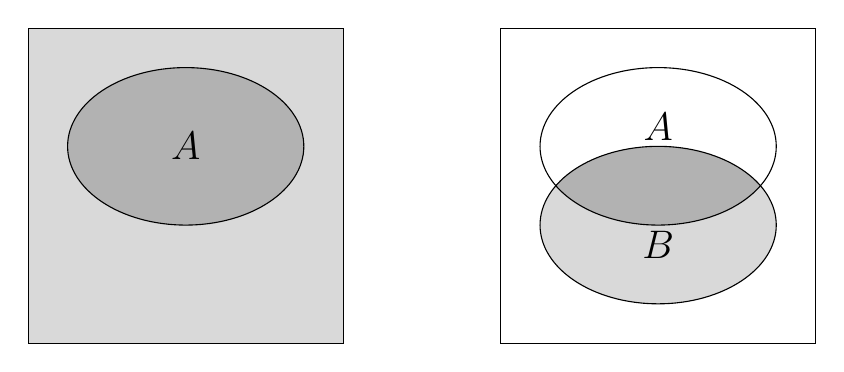
\begin{tikzpicture}
    % Erstes Bild: A in Universalmenge
    \begin{scope}[xshift=0cm]
      % Universalmenge
      \fill[gray!30] (-2,-2) rectangle (2,2);
      \draw (-2,-2) rectangle (2,2);
      % Menge A
      \fill[gray!60] (0,0.5) ellipse (1.5 and 1);
      \draw (0,0.5) ellipse (1.5 and 1);
      \node at (0,0.5) {\Large \(A\)};
    \end{scope}

    % Zweites Bild: A ∩ B hervorgehoben
    \begin{scope}[xshift=6cm]
      \fill[gray!30] (0,-0.5) ellipse (1.5 and 1);
      \draw (-2,-2) rectangle (2,2);
      % Menge A
      \begin{scope}
        \clip (0,0.5) ellipse (1.5 and 1);
        \fill[gray!60] (0,-0.5) ellipse (1.5 and 1);
      \end{scope}

      % Ränder
      \draw (0,0.5) ellipse (1.5 and 1);
      \draw (0,-0.5) ellipse (1.5 and 1);
      % Beschriftungen
      \node at (0,0.75) {\Large \(A\)};
      \node at (0,-0.75) {\Large \(B\)};
    \end{scope}
  \end{tikzpicture}
\end{center}

Die Wahrscheinlichkeit \(P(A)\) ist das Verhältnis von dunkler zu hellgrauer Fläche im Bild links. Die Wahrscheinlichkeit \(P(A\mid B)\) ist das Verhältnis von dunkel- zu hellgrauer Fläche im Bild rechts.

\begin{bsp}
  {}{}
  Alice wirft zwei Würfel und wettet auf das Ereignis \(A:\) `Mindestens eine Sechs'.
  \begin{enumerate}
    \item Was ist ihre Gewinnwahrscheinlichkeit?
    \item Bob schaut unter den Würfelbecher und verrät Alice, dass die Summe der beiden Augenzahlen gleich sieben ist. Wie gross ist nun die Wahrscheinlichkeit, dass Alice gewinnt?
  \end{enumerate}
  \vspace*{6cm}
\end{bsp}



\clearpage
\begin{bsp}
  {Medizinische Tests}{}
  Bei Infektionskrankheiten ist es wichtig, dass man schnell die Art der Krankheit erkennt. Zu diesem Zweck werden heute Schnelltests durchgeführt. Die Güte der Tests wird durch zwei Grössen angegeben: Die \emph{Sensitivität} gibt die Wahrscheinlichkeit an, mit der eine kranke Person positiv getestet wird. Die \emph{Spezifität} gibt an, welcher Anteil der gesunden Personen negativ getestet wird.

  Der ELISA-Test ist ein gängiges Verfahren, um HIV im menschlichen Körper nachzuweisen. Die Sensitivität liegt bei 99.9\%, während die Spezifität 99.7\% beträgt. Laut UNAIDS ist in Westeuropa etwa 0.2\% der Bevölkerung HIV-infiziert.

  Eine Person wird positiv getestet. Mit welcher Wahrscheinlichkeit ist sie HIV-infiziert?

  \vspace*{17cm}

\end{bsp}




\begin{bsp}
  {Zwei Bäume helfen bei der Übersicht}{chorverteilung}
  Ein Chor besteht zu 60\% aus Frauen. 42\% aller Chormitglieder sind älter als 60 Jahre, unter den Männern sind es sogar 60\%.
  \begin{enumerate}
    \item Welcher Prozentsatz der Frauen ist jünger als 60 Jahre?
    \item Ein junges Chormitglied betritt das Probelokal. Mit welcher Wahrscheinlichkeit ist es eine Frau?
  \end{enumerate}
  \vspace*{15 cm}
\end{bsp}
\clearpage
\begin{bsp}
  {Schon mal in Mathe gespickt?}{}
  Der Lehrer möchte herausfinden, wie viele Schüler schon einmal in einer Mathematik-Prüfung abgeschrieben haben. Wird diese Frage direkt gestellt, werden wohl viele nicht die Wahrheit sagen.

  Um die Anonymität zu gewährleisten, gibt es folgende Methode: Jede befragte Person wirft einen Würfel, ohne dass der Lehrer das Ergebnis sieht. Ist die Augenzahl 1 oder 2, wird die Frage beantwortet «Stimmt es, dass du schon einmal in Mathe gespickt hast?». Anderenfalls wird die Frage beantwortet «Stimmt es, dass du in Mathe noch nie gespickt hast?»

  Das Experiment wird in der Klasse durchgeführt und ausgewertet :).

  \vspace*{17cm}

\end{bsp}

\clearpage
\begin{ueb}
  {Medizinische Tests}{}
  \begin{enumerate}


    \item Man weiss, dass 1\% einer Population eine bestimmte Krankheit haben. Ein Test liefert bei 95\% der Kranken und 99.5\% der Gesunden die richtige Diagnose. Bei einer Person diagnostiziert der Test die Krankheit.\\
          Mit welcher Wahrscheinlichkeit ist diese Person gesund?

    \item Eine Krankheit kommt bei 0.1\% einer Population vor. Ein Test reagiert positiv bei 98\% der Kranken, allerdings auch fälschlicherweise bei 5\% des gesunden Teils der Population.\\
          Wie gross ist die Wahrscheinlichkeit, dass eine Person mit positivem Test diese Krankheit hat?

          %   \item Die Wahrscheinlichkeit, dass eine beliebige erwachsene Person an Dickdarmkrebs erkrankt ist, beträgt 0.3\%.\\
          %   Ein Test fällt bei der Hälfte der Personen mit Dickdarmkrebs positiv aus, bei Personen ohne Dickdarmkrebs fälschlicherweise in 3\% aller Fälle.\\
          %   Mit welcher Wahrscheinlichkeit hat eine Person mit positivem Test Dickdarmkrebs?

          %   \item Die Entstehung von Magengeschwüren wird stark von einem bestimmten Bakterium beeinflusst, das recht häufig bei Personen im Alter von 20 bis 40 verbreitet ist. Ein Test zum Nachweis dieses Bakteriums (es heisst Helicobacter Pylori) ist positiv bei 98\% der Personen, die mit diesem Bakterium infiziert sind; er ist negativ bei 97\% der nicht infizierten Personen.\\
          %   Die Wahrscheinlichkeit, dass eine Person mit positivem Testresultat mit dem Bakterium infiziert ist, beträgt 89\%.\\
          %   Wie viele Prozent der Personengruppe 20 bis 40 sind mit dem Bakterium infiziert?

    \item Ein HIV-Test reagiert bei HIV-positiven Personen mit 99\% Wahrscheinlichkeit positiv, allerdings auch bei 3\% der HIV-negativen Personen.\\
          Nun sind 67\% der positiven Testresultate Fehlalarme.\\
          Wie gross ist der Anteil der HIV-positiven Personen unter den getesteten Personen?
          \setcounter{tempCounter}{\value{enumi}}
  \end{enumerate}

\end{ueb}







\begin{ueb}
  {Nach \Cref*{bsp:chorverteilung}}{}
  Tipp: Häufig ist es hilfreich, für jede Aufgabe zwei Bäume zu zeichnen und die gegebenen Wahrscheinlichkeiten einzutragen.
  \begin{enumerate}
    \setcounter{enumi}{\value{tempCounter}}
    \item Bei einer Tombola gewinnt jedes vierte Los. Es werden rote und blaue Lose verkauft. 30\% der Lose sind blau und von ihnen ist jedes dritte Los ein Gewinnlos. Ein Los wird gezogen.
          \begin{enumerate}
            \item Das los ist rot. Mit welcher Wahrscheinlichkeit gewinnt es?
            \item Das Los gewinnt. Mit welcher Wahrscheinlichkeit ist es rot?
          \end{enumerate}




    \item Der Hund eines Zollbeamten bellt, wenn er Rauschgift erschnuppert. Er entdeckt 98\% aller Rauschgift-Schmuggelfälle. In 3\% der Fälle bellt der Hund, obwohl kein Rauschgift geschmuggelt wurde. Die Erfahrung zeigt ausserdem, dass in 1\% aller Grenzübertritte Rauschgift geschmuggelt wird.
          \begin{enumerate}
            \item Wie gross ist die Wahrscheinlichkeit, dass der Hund bellt, wenn er einen Grenzgänger beschnuppert?
            \item Der Hund bellt bei einem Grenzgänger. Wie gross ist die Wahrscheinlichkeit, dass der Grenzgänger tatsächlich Rauschgift schmuggelt?
          \end{enumerate}

    \item Etwa 70\% aller versendeten E-Mails sind Spam. In 80\% dieser Spammails kommt das Wort «free» vor. Dein lernfähiger Spamfilter hat in den letzten Jahren alle deine erhaltenen E-Mails (sowohl Spam als auch Nicht-Spam) durchsucht und fand das Wort «free» in 6 von 10 E-Mails. Nun kommt eine neue E-Mail an, die das Wort «free» enthält. Wie gross ist die Wahrscheinlichkeit, dass es sich bei der E-Mail um Spam handelt?

    \item  Bricht ein Feuer aus, so wird es vom Brandmelder in 99\% aller Fälle erkannt und der Feueralarm wird ausgelöst. Ein Feuer an einer Schule ist jedoch höchst unwahrscheinlich. Die Wahrscheinlichkeit, dass an einem Tag ein Feuer ausbricht, beträgt nur 0.01\%. Die Wahrscheinlichkeit, dass an einem Tag der Feueralarm ertönt, liegt allerdings bei 0.5\%. Wie gross ist die Wahrscheinlichkeit, dass es sich bei einem ausgelösten Alarm um einen Fehlalarm handelt?

  \end{enumerate}
\end{ueb}

\clearpage
\emph{Lösungen}
\begin{enumerate}
  \item ca. 34\%
  \item ca. 1.92\%
        % \item ca. 1.5\%
        % \item ca. 2\%
  \item ca. 1.47\%

  \item 3/14 und 3/5
  \item ca. 4\% und 25\%
  \item 0.933
  \item 0.98
\end{enumerate}












\clearpage
\subsection{Vermischte Übungen}
\begin{ueb}
  {}{}
  \begin{enumerate}


    \item Alice und Bob besuchen ein Fest des Kaninchenzüchtervereins. Dieser bietet eine Lotterie an:  ``Jedes dritte Los gewinnt!''\\
          Die beiden kaufen zusammen fünf Lose. Wie gross ist die Wahrscheinlichkeit,
          \begin{enumerate}
            \item genau einen Gewinn zu realisieren,
            \item \emph{mindestens} einen Gewinn zu realisieren?
          \end{enumerate}

    \item Ein homogener Würfel wird viermal geworfen. Mit welcher Wahrscheinlichkeit zeigt er nur \emph{einmal} die Augenzahl 2?

    \item An der Herbstmesse geben Alice, Bob, Cedric und Dora je einen Schuss auf ein bewegliches Ziel ab. Sie treffen mit den Wahrscheinlichkeiten \\
          \( P(A) = \frac{3}{4}, \quad P(B) = \frac{1}{2}, \quad P(C) = \frac{2}{5}, \quad P(D) = \frac{1}{3} \).\\
          Berechne die Wahrscheinlichkeit, dass
          \begin{enumerate}
            \item alle treffen,
            \item nur C trifft,
            \item das Ziel getroffen wird.
          \end{enumerate}

    \item Eine Urne enthält drei rote und sieben weisse Kugeln; ein Vorrat an Kugeln befindet sich ausserhalb der Urne.\\
          Eine Kugel wird zufällig gezogen, ihre Farbe notiert. Dann legt man vom Vorrat eine Kugel der anderen Farbe in die Urne und zieht nochmals.\\
          Wie gross ist die Wahrscheinlichkeit, dass
          \begin{enumerate}
            \item die zuletzt gezogene Kugel rot ist,
            \item beide Kugeln gleichfarbig sind?
          \end{enumerate}

    \item Eine Urne enthält zwei ``normale'' Münzen und eine Spezialmünze, die auf beiden Seiten \emph{Wappen} zeigt.\\
          Eine Münze wird zufällig gezogen und zweimal geworfen; sie zeigt zweimal \emph{Wappen}.\\
          Mit welcher Wahrscheinlichkeit wurde die Spezialmünze geworfen?


    \item Urne I enthält vier rote und sechs blaue, Urne II fünf rote und vier grüne Kugeln. Ich werfe einen Würfel; zeigt er 1 oder 2, greife ich in die Urne I, andernfalls in die Urne II. Dann ziehe ich aus der so bestimmten Urne nacheinander zwei Kugeln. Dabei lege ich die erste Kugel \emph{nicht} in die Urne zurück.\\
          Wie gross ist die Wahrscheinlichkeit, dass die beiden Kugeln
          \begin{enumerate}
            \item gleichfarbig sind,
            \item verschiedenfarbig sind?
            \item Die Kugeln sind gleichfarbig. Mit welcher Wahrscheinlichkeit sind sie \emph{nicht} rot?
          \end{enumerate}


    \item In einer Urne sind neun rote, vier weisse und einige schwarze Kugeln. Zwei Kugeln werden miteinander gezogen. Sie sind mit der Wahrscheinlichkeit \( \frac{7}{18} \) gleichfarbig.\\
          Wie viele Kugeln sind schwarz?

    \item Ein Portemonnaie enthält total 16 Geldstücke, alle zu 5 Rappen oder 50 Rappen. Rebecca nimmt blindlings zwei Geldstücke heraus. Die Wahrscheinlichkeit, die Summe von 10 Rp. herauszuholen, beträgt \( \frac{3}{8} \).\\
          Wie gross wäre die Wahrscheinlichkeit, die Summe von 55 Rp. herauszuholen?

    \item Bei einem Glücksspiel beträgt die Gewinnwahrscheinlichkeit für den Einzelversuch \( p = \frac{1}{3} \). Ein Spieler macht drei (voneinander unabhängige) Versuche, das Spiel zu gewinnen.
          \begin{enumerate}
            \item Mit welcher Wahrscheinlichkeit gewinnt der Spieler mindestens einmal?
            \item Wie viele Versuche müsste er mindestens machen, um mit einer Wahrscheinlichkeit von über 99\% mindestens einmal zu gewinnen?
          \end{enumerate}

    \item Eine Urne enthält weisse und rote Kugeln. Man stellt fest: Wird eine Kugel gezogen, ist sie mit der Wahrscheinlichkeit \( \frac{1}{3} \) weiss; werden zwei Kugeln gezogen (ohne Zurücklegen), sind sie mit der Wahrscheinlichkeit \( \frac{1}{10} \) weiss.\\
          Wie viele rote und weisse Kugeln enthält die Urne?\\
          Tipp: Diese Aufgabe ist etwas kniffliger. Verwende ein Gleichungssystem mit zwei Unbekannten.

    \item Einer von vier Würfeln, die sich äusserlich nicht unterscheiden, ist manipuliert; bei ihm tritt die Augenzahl 6 mit der Wahrscheinlichkeit 0.3 auf, alle anderen Augenzahlen mit gleicher Wahrscheinlichkeit.\\
          Zufällig wird einer der vier Würfel genommen und zweimal geworfen. Er zeigt die Augensumme 10.\\
          Mit welcher Wahrscheinlichkeit ist es der manipulierte Würfel?\\
          Tipp: Ein Zwischenresultat ist die Wahrscheinlichkeit mit dem manipulierten Würfel die Augensumme 10 zu erhalten. Sie beträgt \(\frac{259}{2500}\).
  \end{enumerate}

\end{ueb}
\clearpage
\emph{Lösungen:}
\begin{enumerate}
  \item a) 80/243, b) 211/243
  \item 125/324
  \item a) 1/20, b) 1/30, c) 19/20
  \item a) 17/50, b) 12/25
  \item 2/3
  \item a) 61/135, b) 74/135, c) 30/61
  \item 15
  \item 1/2
  \item a) 19/27, b) mindestens 12
  \item  14 rote, 7 weisse
  \item ca 0.293
\end{enumerate}